\documentclass[titlepage,a4paper,oneside]{article}
\usepackage[utf8]{inputenc}
\usepackage{amsmath}
\usepackage{mathabx}
\usepackage{graphicx}
\usepackage{minted}
\usepackage{booktabs}
\usepackage[english,spanish,es-noindentfirst,es-nosectiondot,es-nolists,
es-noshorthands,es-lcroman,es-tabla]{babel}
\usepackage{lmodern}             % Use Latin Modern fonts
\usepackage[T1]{fontenc}         % Better output when a diacritic/accent is used
\usepackage[utf8]{inputenc}      % Allows to input accented characters
\usepackage{textcomp}            % Avoid conflicts with siunitx and microtype
\usepackage{microtype}           % Improves justification and typography
\usepackage[svgnames]{xcolor}    % Svgnames option loads navy (blue) colour
\usepackage[hidelinks,urlcolor=blue]{hyperref}
\hypersetup{colorlinks=true, allcolors=Navy, pdfstartview={XYZ null null 1}}
\newtheorem{lemma}{Lema}
\usepackage[width=14cm,left=3.5cm,marginparwidth=3cm,marginparsep=0.35cm,
height=21cm,top=3.7cm,headsep=1cm, headheight=1.6cm,footskip=1.2cm]{geometry}
\usepackage{csquotes}
\usepackage{biblatex}
\addbibresource{informe.bib}
\usepackage[pdf]{graphviz}


\begin{document}

\begin{titlepage}
\title{
	x.y \-- Simulación \\
    \large Facultad de Ingeniería\\
	Universidad de Buenos Aires
}
\author{
	Mermet, Ignacio Javier\\
	\texttt{98153}
}
\date{Julio 2023}

\maketitle

\end{titlepage}

\tableofcontents

\newpage

\section{Introducción}
En el presente trabajo se hará una Introducción al paper \texit{Beyond Finite Layer Neural Networks: Bridging Deep Architectures and Numerical Differential Equations}\cite{Beyond} de \textit{Lu et. al}.

\subsection{Entrenamiento de redes neuronales muy profundas}
Las redes neuronales convolucionales empezaron a dominar el campo de vision por computadora luego de la introducción de AlexNet \cite{AlexNet} en 2012. Estas redes aprenden \textit{features} junto con un clasificador en un proceso punta a punta.

Distintos papers demuestran la importancia de la profundidad de dichas redes para lograr mejores resultados.

Un problema común a la hora de entrenar redes neuronales muy profundas es la explosión de gradientes, otro es el desvanecimiento de gradientes. El primero se refiere a que los valores de los gradientes a medida que se avanza por la red toman valores progresivamente más grandes, hasta tomar el valor nan. El segundo se refiere al caso contrario, donde los gradientes se vuelven progresivamente más pequeños y tienden a cero, frenando por completo el entrenamiento. En ambos casos, la convergencia de la red se ve afectada. Ambos problemas se hacen más aparentes en redes neuronales muy profundas.

Al aumentar la profundidad de las redes, se evidencia una degradación en el error de aprendizaje. La precisión de la red se satura y luego empeora. Esta saturación no se debe a un error de sobreajuste.



\subsection{Redes residuales}
\cite{ResNet} propone lo que denomina aprendizaje de residuos para resolver el problema de degradacon. Deseando aprender $\mathscr{H}(x)$, dejan que una serie de capas no lineales aprender $\mathscr{F}(x) = \mathscr{H}(x) - x$, de modo de obtener la función original como $\mathscr{F}(x) + x$.

En el paper se muestran resultados experimentales demostrando que redes similares pero sin bloques residuales, que solo acumulan capas, muestran un error de entrenamiento más grande. También muestran que agregando capas (y por ende parametros) esta arquitectura obtiene fácilmente ganancias de precisión.

\section{Paper}

\section{Resultados experimentales}
En esta sección se detallan los resultados de distintos experimentos desarrollados a fin de replicar los resultados expuestos en el paper. A estos efectos, se utiliza el código original y se arma un pipeline de entrenamiento acorde a lo relatado en el paper.

\subsection{CIFAR10}
Los experimentos aquí detallados se realizan utilizando el dataset CIFAR10. Este dataset se compone de 60000 imágenes de 32x32 píxeles con tres canales de color (RGB). Se divide en 50000 imágenes de entrenamiento y 10000 para el set de pruebas.

Siguiendo lo especificado en \S 2.2, se aplican técnicas de image augmentation al dataset de entrenamiento. TODO. En particular, se agrega un padding de 4 píxeles a cada lado, de modo tal que la imagen pasa a tener 40x40 píxeles. Con una probabilidad del 50\% se espeja la imagen horizontalmente. Finalmente, se toma un recorte aleatorio de 32x32 píxeles.

En etapa de pruebas, se toma una vista simple de la imagen original de 32x32. Es importante notar esto dado que el paper de ResNet utiliza otra técnica de evaluación, tomando múltiples vistas de la imagen original.

\subsection{Hiperparámetros relevantes}
A fin de seguir los lineamientos planteados por el paper, se modificó el código original y se implementó un pipeline de entrenamiento con los hiperparámetros especificados. El batch size se configuró como 128 imágenes por batch. Se utiliza SGD como optimizador, con weight decay  configurado como 0.0001 y momentum como 0.9.

\begin{figure}[H]
\centering
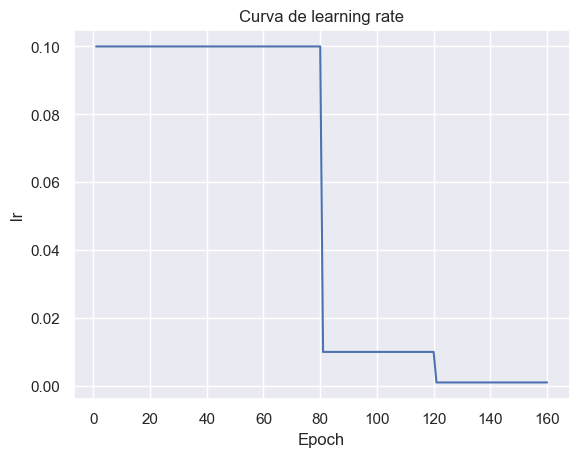
\includegraphics[width=\textwidth]{images/lr_curve.png}
\caption{Curva de learning rate}
\end{figure}

\printbibliography

\end{document}
